\begin{figure}
  \centering
  \begin{subfigure}{0.45\textwidth}
    \centering
    \begin{tikzpicture}
      \node[inner sep=0pt] (img1) at (0,0)
           {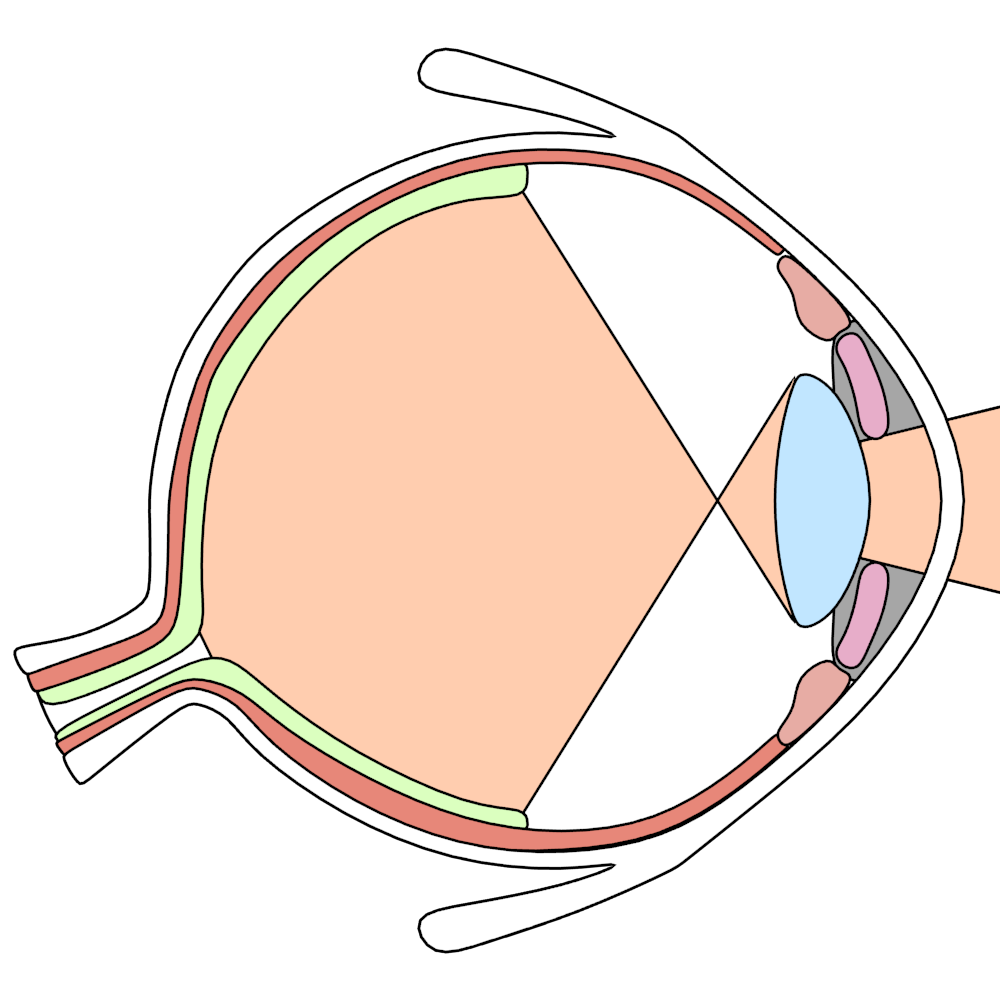
\includegraphics[width=0.9\textwidth]{./img/raw/fw-waarneming/oog.png}};
           
      \node (ret-p) at (-0.27\textwidth, -0.1\textwidth) [] {};
      \node (ret-text) at (-0.27\textwidth, -0.36\textwidth) [] {Retina};
      \draw[-] (ret-p.south) -- (ret-text.north);

      \node (lens-p) at (0.28\textwidth, -0.1\textwidth) [] {};
      \node (lens-text) at (0.28\textwidth, -0.36\textwidth) [] {Lens};
      \draw[-] (lens-p.south) -- (lens-text.north);
    \end{tikzpicture}
    \caption{Oog.}
    \label{fig:fw-waarneming:oog}
  \end{subfigure}%
  \begin{subfigure}{0.45\textwidth}
    \centering
    \begin{tikzpicture}
      \node[inner sep=0pt] (img1) at (0,0)
           {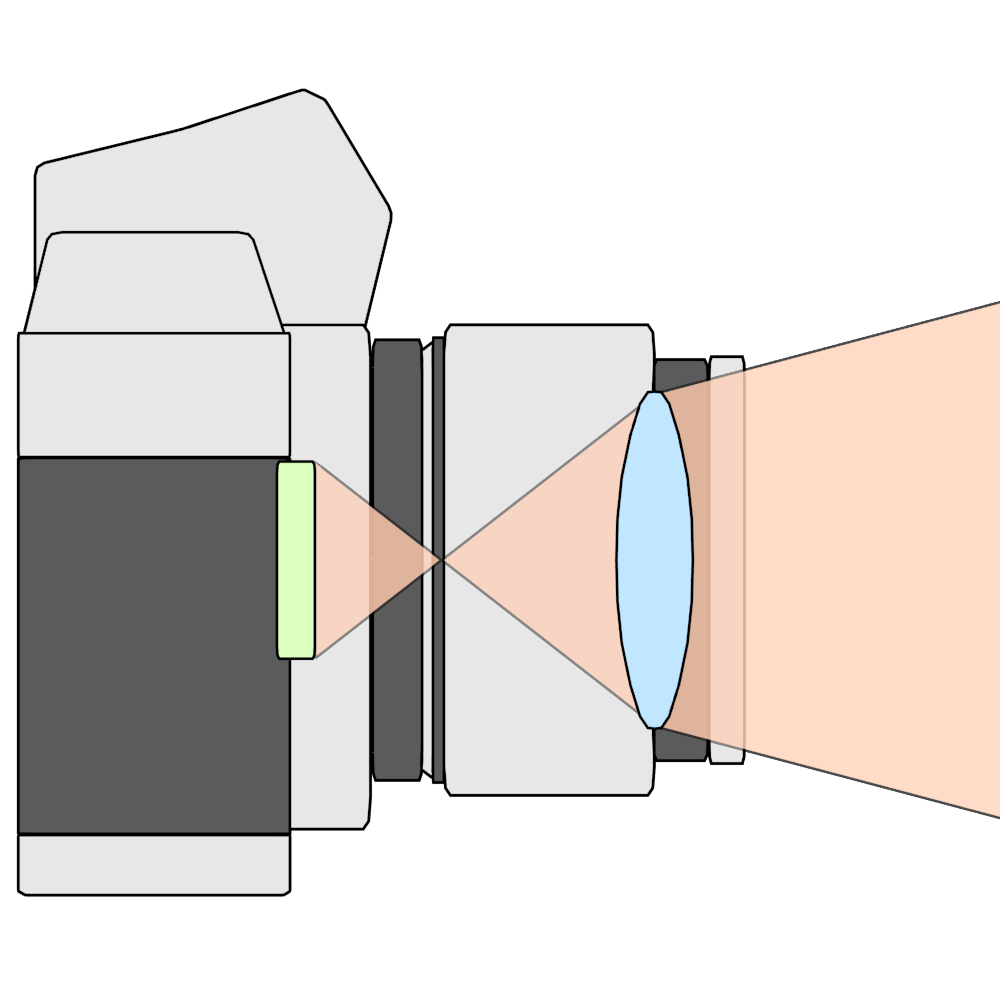
\includegraphics[width=0.9\textwidth]{./img/raw/fw-waarneming/camera.png}};   

      \node (sensor-p) at (-0.185\textwidth, -0.13\textwidth) [] {};
      \node (sensor-text) at (-0.05\textwidth, -0.36\textwidth) [] {Sensor};
      \draw[-] (sensor-p.south) -- (sensor-text.north);

      \node (lens-p) at (0.146\textwidth, -0.19\textwidth) [] {};
      \node (lens-text) at (0.28\textwidth, -0.36\textwidth) [] {Lens};
      \draw[-] (lens-p.south) -- (lens-text.north);
    \end{tikzpicture}
    \caption{Camera.}
    \label{fig:fw-waarneming:oog}
  \end{subfigure}
  \caption{Waarneming door middel van het oog en camera.}
  \label{fig:fw-waarneming}
\end{figure}
